\section{Κωδικοποίηση \& Αποκωδικοποίηση Huffman}



\noindent
\begin{minipage}{\linewidth}
\par Το επόμενο βήμα για την υλοποίηση του συστήματος Κωδικοποιητή και Αποκωδικοποιητή που θέλουμε να
αναπτύξουμε είναι η κωδικοποίηση των συμβόλων που αποτελούν το σήμα μας και για αυτό το σκοπό
στρεφόμαστε στην χρήση του κώδικα Huffman.

  \par Ο αλγόριθμος του Huffman βασίζεται στις πιθανότητες εμφάνισης των συμβόλων που μας ενδιαφέρουν
  προκειμένου να εξάγει τον κώδικα που θα χρησιμοποιήσουμε για συμπίεση. Συγκεκριμένα, όσο πιο πιθανό
  είναι ένα σύμβολο, τόσο μικρότερη είναι η συμβολοσειρά που το αναπαριστά. Πρακτικά, μπορεί να
  αναπαρασταθεί από ένα δυαδικό δέντρο, όπου τα φύλλα αντιστοιχούν στα σύμβολα. Για την κατασκευή του
  δέντρου, ξεκινάμε από δύο στοιχεία που έχουν τη μικρότερη πιθανότητα, τα οποία κι ενώνουμε για να
  σχηματίσουμε έναν κόμβο του δέντρο, ο οποίος με την σειρά του θεωρείται ως ένα νέο σύμβολο, με
  πιθανότητα ίση με το άθροισμα των πιθανοτήτων των παιδιών. Στην συνέχεια, επιλέγουμε τα στοιχεία που
  έχουν τις δύο μικρότερες πιθανότητες κι επαναλαμβάνουν την παραπάνω διαδικασία. Ο αλγόριθμος
  τερματίζει όταν όλοι οι κόμβοι έχουν ενωθεί.
  \begin{framed}
    \begin{figure}[H]
      \label{fig:huffman}
      \centering
      \begin{subfigure}{1.0\textwidth}
        \centering
        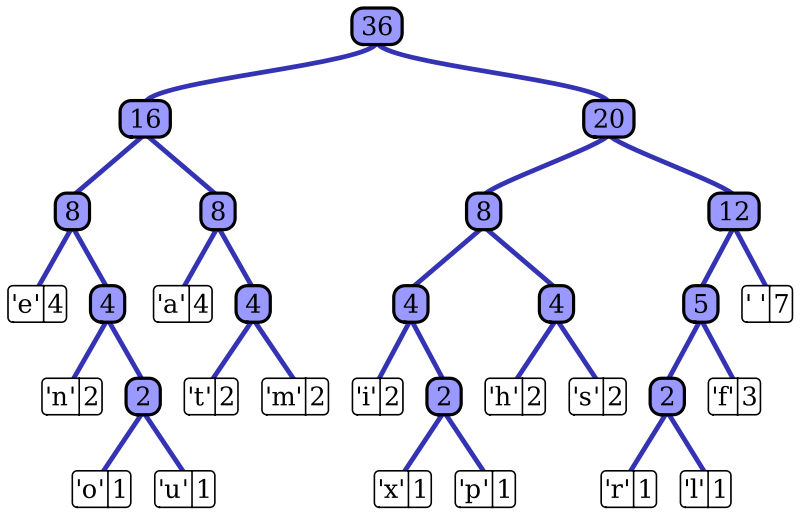
\includegraphics[width=0.8\textwidth]{huffman}
        \caption{\protect{Πηγή: \href{https://en.wikipedia.org/wiki/Huffman\_coding}{Huffman Wikipedia Article}}}
      \end{subfigure}
      \caption{Παράδειγμα Δέντρου Huffman}
    \end{figure}
  \end{framed}
\end{minipage}

\par Η συνάρτηση που κατασκευάζει το παραπάνω δέντρο και κατά συνέπεια και το λεξικό/σύνολο λέξεων
που μας δίνει τον κώδικα Huffman είναι η:
\begin{lstlisting}[style=myMatlab]
  function [s] = huffLUT(p, debug)
\end{lstlisting}
\noindent η οποία αρχικά δημιουργεί μία ουρά προτεραιότητας με κόμβους, όπου κάθε κόμβος είναι ένα
φύλλο που περιέχει ένα από τα αρχικά σύμβολα. Έπειτα, και για όσο υπάρχουν στοιχεία στην ουρά,
εξάγουμε τα δύο στοιχεία με τις χαμηλότερες πιθανότητες, τα ενώνουμε δημιουργώντας έναν νέο κόμβο,
όπως περιγράψαμε παραπάνω και τον οποίο εισάγουμε στην ουρά, αναθέτοντας του και το αντίστοιχο
ψηφίο. Για να εξάγουμε τον κώδικα που αντιστοιχεί σε κάθε σύμβολο, απλά ξεκινάμε από το αντίστοιχο
φύλλο κι ανεβαίνουμε μέχρι την ρίζα του δέντρου, κρατώντας τα ψηφία των κόμβων από τους οποίους
περνάμε.

\par Η συνάρτηση:
\begin{lstlisting}[style=myMatlab]
  function [b] = huff(q, s)
\end{lstlisting}
\noindent κωδικοποιεί την συμβολοσειρά που μας δίνεται με βάση το λεξιλόγιο που δημιούργησε η
\emphcolor{huffLut} αντιστοιχώντας κάθε σύμβολο στον κώδικα του.

\par Τέλος, η συνάρτηση:
\begin{lstlisting}[style=myMatlab]
  function [q, n] = ihuff(b, s, debug)
\end{lstlisting}
\noindent εκτελεί τον αντίστροφο μετασχηματισμό Huffman δοθέντος του λεξιλογίου και μίας σειράς
ψηφίων. Για να το πετύχει αυτό δημιουργεί το δέντρο Huffman από τις κωδικολέξεις, εκτελώντας
έναν βρόγχο for για κάθε μία από αυτές. Αρχικά, δημιουργούμε έναν κενό κόμβο, ο οποίος και αποτελεί
την ρίζα του δέντρου μας. Στην συνέχεια, για κάθε κωδικολέξη, εξετάζουμε ένας προς ένα τα ψηφία της
και δημιουργούμε έναν νέο κόμβο για το καθένα εφόσον δεν υπάρχει, στα δεξιά τρέχοντος κόμβου αν
είναι το 0, διαφορετικά στα αριστερά, προχωρώντας μέχρι να εξαντλήσουμε τα bits της. Όταν εξετάσουμε
το σύνολο του λεξιλογίου θα έχουμε κατασκευάσει ξανά το δέντρο Huffman.
\par Προκειμένου να αποκωδικοποιήσουμε το bitstream που μας δίνεται, εισάγουμε τα bits του στο
δέντρο. Μόλις βρεθούμε σε κάποιο φύλλο προσθέτουμε στο τέλος της αποκωδικοποιημένης πρότασης μας το
αντίστοιχο σύμβολο. Αν στο τέλος της σειράς των bits δεν βρισκόμαστε σε φύλλο τότε επιστρέφουμε και
τον αριθμό των μηδενικών και άσσων που περίσσεψαν.
